\section*{Introduction}
Soit une poutre de section carré et de longueur "infinie" soumise à une charge $F$. On se propose d'étudier la résistance de cette poutre lorsqu'elle est chargée verticalement. On définie le champs de contraintes $\sigma = \begin{pmatrix}
\sigma_{xx} & \sigma_{xy}\\
\sigma_{xy} & \sigma_{yy}
\end{pmatrix}$. On souhaite maximiser la charge imposé (c'est à dire l'intégrale de $\sigma_{yy}$ sur la surface supérieur de la poutre) sans qu'il y ait déformation plastique, sous les contraintes mécaniques suivantes : 
\begin{align}
\frac{\partial \sigma_{xx}}{\partial x} + \frac{\partial \sigma_{xy}}{\partial y} &= 0 \label{eq:contrainteequilibre1}\\
\frac{\partial \sigma_{xy}}{\partial x} + \frac{\partial \sigma_{yy}}{\partial y} &= 0\label{eq:contrainteequilibre2}\\
\sigma^{(i)}n &= \sigma^{(j)}n & \text{si le triangles $(i)$ et $(j)$ ont un côté de normale $n$ en commun} \label{eq:contrainteContinuite}\\
\sigma n &= 0 & \text{sur la frontière} \label{eq:contrainteFrontiere}
\end{align}
où les contraintes \eqref{eq:contrainteequilibre1} et \eqref{eq:contrainteequilibre2} expriment la conservation de la quantité de mouvement. \\
Comme ce problème possède une infinité de contraintes (problème continu), nous le discrétisons en triangles comme à la figure \ref{fig:discretisation}. A première vue, un noeud peut prendre plusieurs valeurs $\sigma$ si il appartient à plusieurs triangles. 

\begin{figure}
\centering
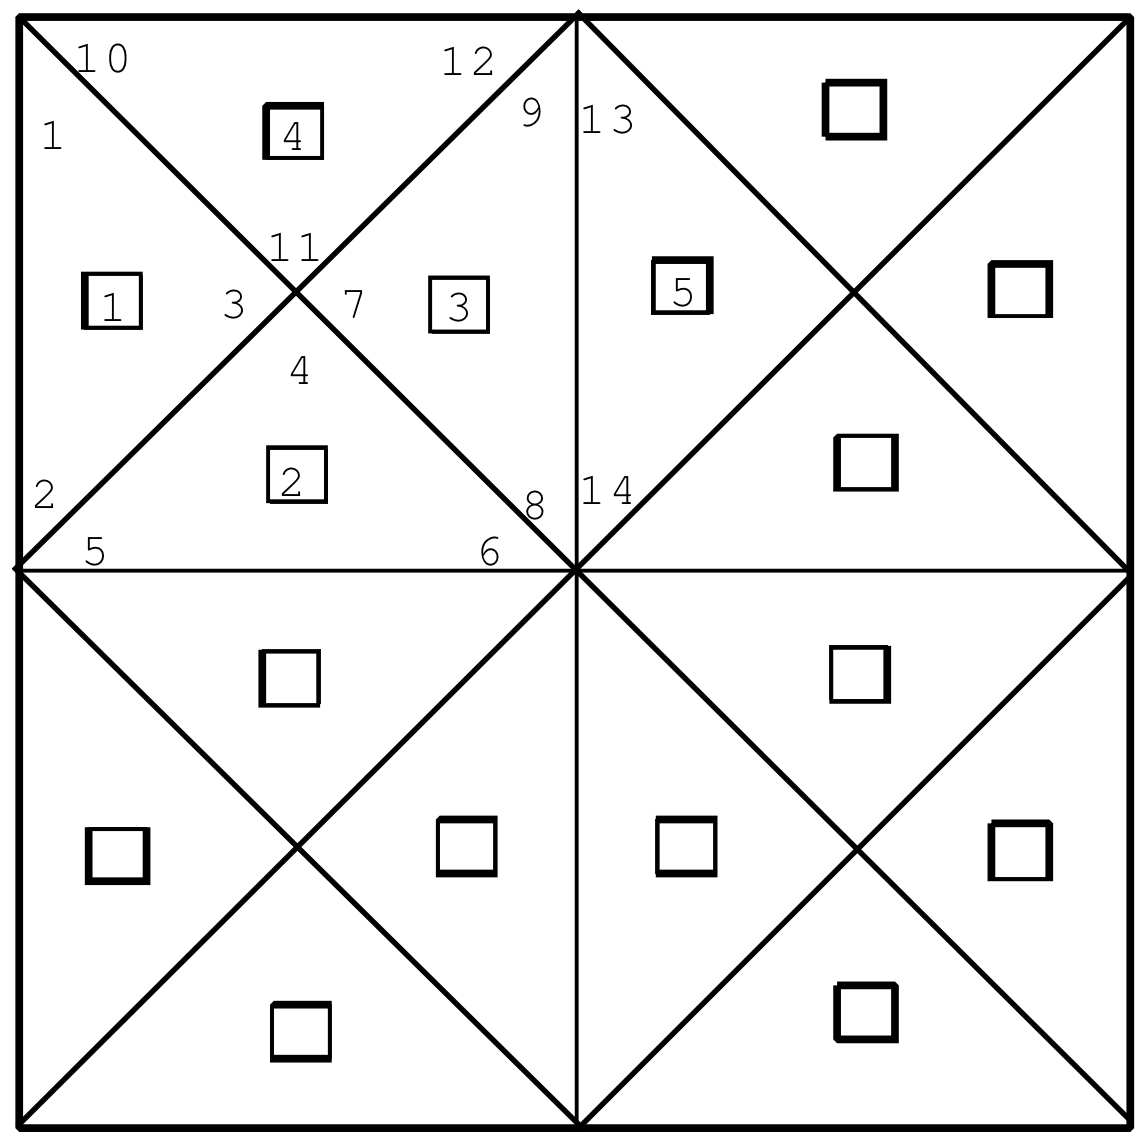
\includegraphics[height=5cm]{images/discretisation.png}
\caption{Section de la poutre discrétisée en triangles}
\label{fig:discretisation}
\end{figure}


\newpage
\section{Modélisation}
On peut modéliser notre problème comme un problème d'éléments finis. Nos variables sont les $\sigma_{xx}^i$, $\sigma_{xy}^i$ et $\sigma_{yy}^i$ en chaque nœud $i$. Nous interpolons linéairement le champ des contraintes dans chaque triangles $k$.
Afin de définir facilement nos fonctions de formes, on effectue un changement de variables $(x,y)\rightarrow (\xi,\eta)$ où $(\xi, \eta)$ sont les coordonnées dans le triangle parents (de sommets $(0,0)$, $(1,0)$ et $(0,1)$). 
Soit un triangle quelconque dont les points sont numéroté $m,n,p$. 
Le gradient ce la transformation $\frac{\partial (\xi,\eta)}{\partial (x,y)}$ est donné par  : $\frac{\partial \xi}{\partial x} = \frac{1}{x_m - x_n}$, $\frac{\partial \xi}{\partial y} = \frac{1}{y_m - y_n}$, $\frac{\partial \eta}{\partial x} = \frac{1}{x_p - x_m}$ et $\frac{\partial \eta}{\partial y} = \frac{1}{y_p - y_m}$
Chacun des champs sur un triangle $k$ est défini comme suit : 
\begin{equation} \label{eq:champsEFM}
\begin{aligned}
\sigma_{xx}^k (\xi,\eta) &= \sum_{j \in \{\text{noeud de $k$}\}} \phi_j (\xi,\eta) \sigma_{xx}^{k,j}\\
\sigma_{xy}^k (\xi,\eta) &= \sum_{j \in \{\text{noeud de $k$}\}} \phi_j (\xi,\eta) \sigma_{xy}^{k,j}\\
\sigma_{yy}^k (\xi,\eta) &= \sum_{j \in \{\text{noeud de $k$}\}} \phi_j (\xi,\eta) \sigma_{yy}^{k,j}
\end{aligned}
\end{equation}
où les $\phi_j$ sont les fonctions de formes suivantes : 
\begin{equation}
\begin{aligned}
\phi_1 (\xi,\eta) &= (1- \xi - \eta)\\
\phi_2 (\xi,\eta) &= \xi\\
\phi_3 (\xi,\eta) &= \eta
\end{aligned}
\end{equation}
On impose ensuite nos contraintes \eqref{eq:contrainteequilibre1}, \eqref{eq:contrainteequilibre2}, \eqref{eq:contrainteContinuite} et \eqref{eq:contrainteFrontiere} sur nos champs définis comme en \eqref{eq:champsEFM}. 
Dans notre cas, comme les triangles sont rectangle, ces expressions se simplifient fortement. On utilise la "chain rule" pour exprimer les dérivées partielles de \eqref{eq:contrainteequilibre1} et \eqref{eq:contrainteequilibre2}, par example : $\frac{\partial \sigma_{xx}}{\partial x} = \frac{\partial \sigma_{xx}}{\partial \xi} \frac{\partial \xi}{\partial x} + \frac{\partial \sigma_{xx}}{\partial \eta} \frac{\partial \eta}{\partial x}$. On obtient les expressions suivantes : 
\begin{align}
& \max ??? \\
\frac{\sigma_{xx}^n - \sigma_{xx}^m}{x_m - x_n}  + \frac{\sigma_{xx}^p - \sigma_{xx}^m}{x_p - x_m} + \frac{\sigma_{xy}^n - \sigma_{xy}^m}{y_n - y_m} + \frac{\sigma_{xy}^p - \sigma_{xy}^m}{y_p - y_m} &= 0  & \forall \triangle j, \forall \text{noeud $m$, $n$ et $p$} \in \triangle_j \\
\frac{\sigma_{xy}^n - \sigma_{xy}^m}{x_m - x_n}  + \frac{\sigma_{xy}^p - \sigma_{xy}^m}{x_p - x_m} + \frac{\sigma_{yy}^n - \sigma_{yy}^m}{y_n - y_m} + \frac{\sigma_{yy}^p - \sigma_{yy}^m}{y_p - y_m} &= 0  & \forall \triangle j, \forall \text{noeud $m$, $n$ et $p$} \in \triangle_j \\
\sigma_{xx}^i &= \sigma_{xx}^j & \text{si le noeud (i) et (j) sont confondus}\\
\sigma_{xy}^i &= \sigma_{xy}^j & \text{si le noeud (i) et (j) sont confondus}\\
\sigma_{yy}^i &= \sigma_{yy}^j & \text{si le noeud (i) et (j) sont confondus}\\
\sigma_{xx}^i &= 0 & \text{si le noeud (i) est sur la frontière} \\
\sigma_{xy}^i &= 0 & \text{si le noeud (i) est sur la frontière}\\
\sigma_{yy}^i &= 0 & \text{si le noeud (i) est sur la frontière}
\end{align}




